\documentclass[../main.tex]{subfile}

\begin{document}

\section{Численные методы интегрирования}

Как мы находили определённый интеграл от функции $f(x)$ на отрезке $[a,b]$? Мы
всевозможными способами искали первообразную $F(x)$, а затем по формуле
Ньютона-Лейбница $\int_a^bf(x)dx=F(b)-F(a)$ вычисляли его значение. И эта
формула работала.

Проблемы начинаются тогда, когда у функции не получается найти первообразную
или она выглядит слишком сложно или страшно, чтобы в неё что-то там подставлять.
Наконец, функция может быть задана таблично, а не аналитической функцией.

Это значит, что отталкиваться придётся только от исходной функции $f(x)$. О том,
как приближённо найти интеграл без первообразной, и будет рассказано в этой главе.

\begin{define}
	\textbf{Задача численного интегрирования} -- задача нахождения
	определённого интеграла функции без использования её первообразной и
	формулы Ньютона-Лейбница.
\end{define}

Наиболее часто для численного интегрирования используется следующая формула.

\begin{define}\label{eq:quadrature_formula}
	\textbf{Квадратурная формула} -- формула вида
	\[\int_a^bf(x)dx\approx\sum_{k=0}^n c_kf(x_k),\]
	где $c_k$ -- \textbf{весовые коэффициенты}, а $x_k\in[a,b]$ --
	\textbf{узлы интегрирования}.
\end{define}

\begin{define}
	\textbf{Кубатурная формула} -- формула вида
	\[\int_{D}f(x)dx\approx\sum_{k=0}^n c_k f(x_k),\quad x_k\in D,\;D
	\subseteq\mathbb R^m,\;m\ge 2.\]
\end{define}

\begin{define}
	\textbf{Сетка} -- это совокупность узлов $\{x_1,...,x_n\}$ квадратурной
	или кубатурной формулы.
\end{define}

\begin{define}
	\textbf{Погрешность квадратурной формулы} или её \textbf{остаточный
	член} -- это разность
	\[R_{[a,b]}(f)=\int_a^b f(x)dx - \sum_{k=0}^n c_kf(x_k).\]
\end{define}

\begin{define}
	Квадратурная формула называется \textbf{точной} для функции $f$ или
	класса $\mathcal F\ni f$ на интервале $[a,b]$, если верно $R_{[a,b]}(f)=0$.
\end{define}

То, насколько широк класс $\mathcal F$, на которых квадратурная формула точна,
может говорить о точности квадратурной формулы в целом. Часто в качестве класса
''пробных'' функций $\mathcal F$ берут алгебраические полиномы.

\begin{define}
	\textbf{Алгебраическая степень точности} квадратурной формулы --
	наибольшая степень алгебраического полинома, для которого эта формула
	точна на всей вещественной оси.
\end{define}

Конечно, для нас предпочтительней формулы с б\'{о}льшей алгебраической степенью
точности.

\subsection{Формулы Ньютона-Котеса}
Простейший приём построения квадратурных формул -- замена подынтегральной
функции $f(x)$ на интервале интегрирования $[a,b]$ на ''более простую'',
легче интегрируемую функцию. Подынтегральную функцию чаще всего интерполируют
алгебраическими полиномами.\newpage

\begin{define}
	\textbf{Интерполяционная квадратурная формула} -- квадратурная формула
	\eqref{eq:quadrature_formula}, которая заменяет исходную функцию $f(x)$
	интерполянтом по простым (то есть не кратным) узлам $\{x_1,...,x_n\}$:
	\[f(x)\approx g(x)=\sum_{k=0}^{n}f(x_k)\gamma_k(x),\]
	где $\gamma_k(x)$ -- некоторые функции. Тогда интеграл приблизительно
	равен
	\[\int_{a}^{b}f(x)dx\approx\sum_{k=0}^{n}f(x_k)
	\underset{c_k}{\underbrace{\int_{a}^{b}\gamma_k(x)dx}}.\]
\end{define}

\begin{define}\label{eq:newton_cotes_formula}
	\textbf{Формула Ньютона-Котеса} -- интерполяционная квадратурная
	формула, полученная с помощью алгебраической интерполяции
	\eqref{eq:interpolating_polynomial} подынтегральной функции на
	равномерной сетке с простыми узлами на отрезке $[a,b]$.
\end{define}

То есть $\gamma_k(x)$ -- это алгебраические полиномы. Мы рассмотрим формулы
замкнутого типа (то есть такие, что границы отрезка интегрирования являются
частью сетки) при $n\in\{0,1,2\}$.

\begin{define}\label{eq:rectangle_formula}
	\textbf{Формула прямоугольников} -- простейшая квадратурная формула
	Нью-тона-Котеса, интерполяционная функция которой задаётся единственным
	узлом $x_0\in[a,b]$ и, следовательно, равна константе. Формула имеет вид
	\[\boxed{\int_{a}^{b}f(x)dx\approx f(x_0)(b-a)}\]
\end{define}

Название идёт из того, что она совпадает с площадью прямоугольника со сторонами
$(b-a)$ и $f(x_0)$. Не нужно забывать, что геометрический смысл интеграла -- это
площадь фигуры под графиком функции.

Несмотря на то что мы писали, что все формулы будут замкнутого типа, это не
касается формулы прямоугольников, потому что для замкнутости не хватает узлов
интерполяции.

\begin{define}
	Если в формуле \eqref{eq:rectangle_formula} $x_0$ такой, что
	\begin{itemize}[noitemsep, nolistsep]
		\item $x_0=a$, это \textbf{формула левого прямоугольника}.
		\item $x_0=b$, это \textbf{формула правого прямоугольника}.
		\item $x_0=\frac{a+b}{2}$, это \textbf{формула среднего
			прямоугольника}.
	\end{itemize}

	На графике эти формулы выглядят вот так:

	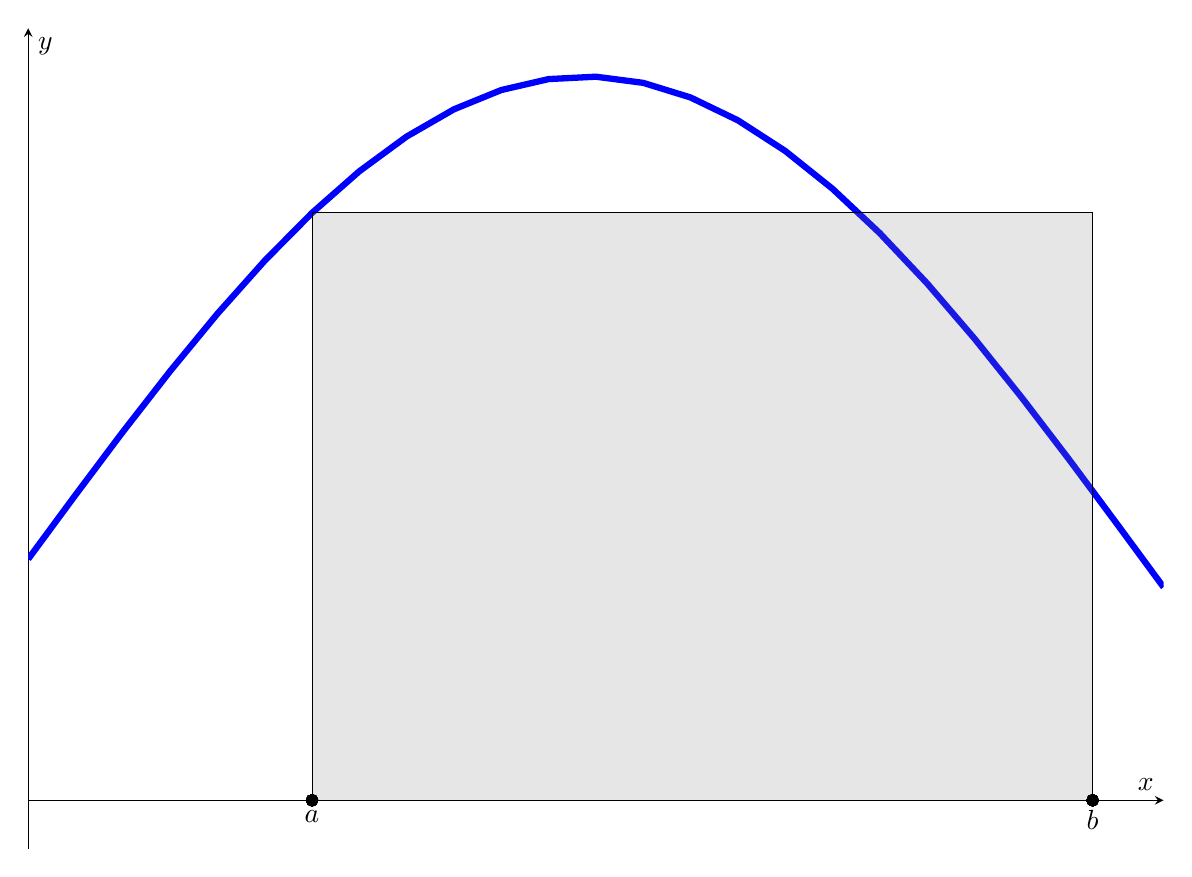
\begin{tikzpicture} [
		declare function={
			f(\x)= sin(\x / pi * 180)+0.5;
		},]
		\begin{axis} [
			height=12cm,
			width=16cm,
			xlabel = {$x$},
			ylabel = {$y$},
			axis x line = middle,
			axis y line = middle,
			ymin = -0.1,
			ymax = 1.6,
			domain = 0:3.2,
			ticks = none ]

			\newcommand*{\varA}{0.8}
			\newcommand*{\varB}{3}
			\pgfmathsetmacro{\fa}{f(\varA)}
			\pgfmathsetmacro{\fb}{f(\varB)}

			\addplot[color=blue, line width=.08cm]{f(x)};

			\coordinate(A) at 	(\varA,		\fa);
			\coordinate(Ap) at 	(\varA,		0);
			\coordinate(B) at 	(\varB,		\fb);
			\coordinate(Bp) at 	(\varB,		0);

			\node[below](Alb) at 	(\varA,		0) {$a$};
			\node[below](Blb) at 	(\varB,		0) {$b$};

			\addplot[mark=*,only marks, fill=black] (\varA, 0)
				node[above, pos=1]{};
			\addplot[mark=*,only marks, fill=black] (\varB, 0)
				node[above, pos=1]{};

			\draw[fill=gray, fill opacity=0.2] (A) rectangle (Bp);
		\end{axis}
	\end{tikzpicture}
\end{define}
\end{document}
